\documentclass[a4paper,11pt,oneside]{memoir}

% Castellano
\usepackage[spanish]{babel}
\selectlanguage{spanish}
\usepackage[utf8]{inputenc}
\usepackage{placeins}

\RequirePackage{booktabs}
\RequirePackage[table]{xcolor}
\RequirePackage{xtab}
\RequirePackage{multirow}

% Links
\usepackage[colorlinks]{hyperref}
\hypersetup{
	allcolors = {red}
}

% Ecuaciones
\usepackage{amsmath}

% Rutas de fichero / paquete
\newcommand{\ruta}[1]{{\sffamily #1}}

% Párrafos
\nonzeroparskip

%color
\usepackage{color}
\definecolor{javapurple}{rgb}{0.5,0,0.35}
\definecolor{pgreen}{rgb}{0,0.5,0}
\definecolor{pred}{rgb}{0.9,0,0}
\definecolor{pgrey}{rgb}{0.46,0.45,0.48}

%Apaisado
\usepackage{lscape}

%Código
\usepackage{listings}
\renewcommand{\lstlistingname}{Código}% Listing -> Algorithm
\renewcommand{\lstlistlistingname}{List of \lstlistingname s}% List of Listings -> List of Algorithms
\usepackage{listings}
\lstset{language=Java,
  showspaces=false,
  showtabs=false,
  breaklines=true,
  showstringspaces=false,
  breakatwhitespace=true,
  commentstyle=\color{pgreen},
  keywordstyle=\color{javapurple}\bfseries,
  stringstyle=\color{pred},
  basicstyle=\ttfamily,
}



%Anotaciones TODO

\usepackage[disable]{todonotes}

%Para el apaisado

\usepackage{lscape}

%Para el posicionamiento correcto de las tablas
\usepackage{float}
\restylefloat{table}

%Para las notas a pie de página dentro de tablas
\usepackage{tablefootnote}

%Para el pseudocódigo

\usepackage[linesnumbered,ruled,vlined,spanish]{algorithm2e}
\usepackage{amssymb}


% Imagenes
\usepackage{graphicx}
\newcommand{\imagen}[2]{
	\begin{figure}[!h]
		\centering
		\includegraphics[width=0.9\textwidth]{#1}
		\caption{#2}\label{fig:#1}
	\end{figure}
	\FloatBarrier
}

\newcommand{\imagenflotante}[2]{
	\begin{figure}%[!h]
		\centering
		\includegraphics[width=0.9\textwidth]{#1}
		\caption{#2}\label{fig:#1}
	\end{figure}
}



% El comando \figura nos permite insertar figuras comodamente, y utilizando
% siempre el mismo formato. Los parametros son:
% 1 -> Porcentaje del ancho de página que ocupará la figura (de 0 a 1)
% 2 --> Fichero de la imagen
% 3 --> Texto a pie de imagen
% 4 --> Etiqueta (label) para referencias
% 5 --> Opciones que queramos pasarle al \includegraphics
% 6 --> Opciones de posicionamiento a pasarle a \begin{figure}
\newcommand{\figuraConPosicion}[6]{%
  \setlength{\anchoFloat}{#1\textwidth}%
  \addtolength{\anchoFloat}{-4\fboxsep}%
  \setlength{\anchoFigura}{\anchoFloat}%
  \begin{figure}[#6]
    \begin{center}%
      \Ovalbox{%
        \begin{minipage}{\anchoFloat}%
          \begin{center}%
            \includegraphics[width=\anchoFigura,#5]{#2}%
            \caption{#3}%
            \label{#4}%
          \end{center}%
        \end{minipage}
      }%
    \end{center}%
  \end{figure}%
}

%
% Comando para incluir imágenes en formato apaisado (sin marco).
\newcommand{\figuraApaisadaSinMarco}[5]{%
  \begin{figure}%
    \begin{center}%
    \includegraphics[angle=90,height=#1\textheight,#5]{#2}%
    \caption{#3}%
    \label{#4}%
    \end{center}%
  \end{figure}%
}
% Para las tablas
\newcommand{\otoprule}{\midrule [\heavyrulewidth]}
%
% Nuevo comando para tablas pequeñas (menos de una página).
\newcommand{\tablaSmall}[5]{%
 \begin{table}[H]
  \begin{center}
   \rowcolors {2}{gray!35}{}
   \begin{tabular}{#2}
    \toprule
    #4
    \otoprule
    #5
    \bottomrule
   \end{tabular}
   \caption{#1}
   \label{tabla:#3}
  \end{center}
 \end{table}
}



%
% Nuevo comando para tablas pequeñas (menos de una página).
\newcommand{\tablaSmallSinColores}[5]{%
 \begin{table}[H]
  \begin{center}
   \begin{tabular}{#2}
    \toprule
    #4
    \otoprule
    #5
    \bottomrule
   \end{tabular}
   \caption{#1}
   \label{tabla:#3}
  \end{center}
 \end{table}
}

\newcommand{\tablaApaisadaSmall}[5]{%
\begin{landscape}
  \begin{table}
   \begin{center}
    \rowcolors {2}{gray!35}{}
    \begin{tabular}{#2}
     \toprule
     #4
     \otoprule
     #5
     \bottomrule
    \end{tabular}
    \caption{#1}
    \label{tabla:#3}
   \end{center}
  \end{table}
\end{landscape}
}

%
% Nuevo comando para tablas grandes con cabecera y filas alternas coloreadas en gris.
\newcommand{\tabla}[6]{%
  \begin{center}
    \tablefirsthead{
      \toprule
      #5
      \otoprule
    }
    \tablehead{
      \multicolumn{#3}{l}{\small\sl continúa desde la página anterior}\\
      \toprule
      #5
      \otoprule
    }
    \tabletail{
      \hline
      \multicolumn{#3}{r}{\small\sl continúa en la página siguiente}\\
    }
    \tablelasttail{
      \hline
    }
    \bottomcaption{#1}
    \rowcolors {2}{gray!35}{}
    \begin{xtabular}{#2}
      #6
      \bottomrule
    \end{xtabular}
    \label{tabla:#4}
  \end{center}
}

%
% Nuevo comando para tablas grandes con cabecera.
\newcommand{\tablaSinColores}[6]{%
  \begin{center}
    \tablefirsthead{
      \toprule
      #5
      \otoprule
    }
    \tablehead{
      \multicolumn{#3}{l}{\small\sl continúa desde la página anterior}\\
      \toprule
      #5
      \otoprule
    }
    \tabletail{
      \hline
      \multicolumn{#3}{r}{\small\sl continúa en la página siguiente}\\
    }
    \tablelasttail{
      \hline
    }
    \bottomcaption{#1}
    \begin{xtabular}{#2}
      #6
      \bottomrule
    \end{xtabular}
    \label{tabla:#4}
  \end{center}
}

%
% Nuevo comando para tablas grandes sin cabecera.
\newcommand{\tablaSinCabecera}[5]{%
  \begin{center}
    \tablefirsthead{
      \toprule
    }
    \tablehead{
      \multicolumn{#3}{l}{\small\sl continúa desde la página anterior}\\
      \hline
    }
    \tabletail{
      \hline
      \multicolumn{#3}{r}{\small\sl continúa en la página siguiente}\\
    }
    \tablelasttail{
      \hline
    }
    \bottomcaption{#1}
  \begin{xtabular}{#2}
    #5
   \bottomrule
  \end{xtabular}
  \label{tabla:#4}
  \end{center}
}



\definecolor{cgoLight}{HTML}{EEEEEE}
\definecolor{cgoExtralight}{HTML}{FFFFFF}

%
% Nuevo comando para tablas grandes sin cabecera.
\newcommand{\tablaSinCabeceraConBandas}[5]{%
  \begin{center}
    \tablefirsthead{
      \toprule
    }
    \tablehead{
      \multicolumn{#3}{l}{\small\sl continúa desde la página anterior}\\
      \hline
    }
    \tabletail{
      \hline
      \multicolumn{#3}{r}{\small\sl continúa en la página siguiente}\\
    }
    \tablelasttail{
      \hline
    }
    \bottomcaption{#1}
    \rowcolors[]{1}{cgoExtralight}{cgoLight}

  \begin{xtabular}{#2}
    #5
   \bottomrule
  \end{xtabular}
  \label{tabla:#4}
  \end{center}
}



\graphicspath{ {./img/} }

% Capítulos
\chapterstyle{bianchi}
\newcommand{\capitulo}[2]{
	\setcounter{secnumdepth}{3}
	\setcounter{chapter}{#1}
	\setcounter{section}{0}
	\chapter*{#2}
	\addcontentsline{toc}{chapter}{#2}
	\markboth{#2}{#2}
}

% Apéndices
\renewcommand{\appendixname}{Apéndice}
\renewcommand*\cftappendixname{\appendixname}

\newcommand{\apendice}[1]{
	%\renewcommand{\thechapter}{A}
	\chapter{#1}
}

\renewcommand*\cftappendixname{\appendixname\ }

% Formato de portada
\makeatletter
\usepackage{xcolor}
\newcommand{\tutorA}[1]{\def\@tutorA{#1}}
\newcommand{\tutorB}[1]{\def\@tutorB{#1}}
\newcommand{\course}[1]{\def\@course{#1}}
\definecolor{cpardoBox}{HTML}{E6E6FF}
\def\maketitle{
  \null
  \thispagestyle{empty}
  % Cabecera ----------------
\noindent
\includegraphics[width=\textwidth]{cabecera}\vspace{1cm}%
  \vfill
  % Título proyecto y escudo informática ----------------
  \colorbox{cpardoBox}{%
    \begin{minipage}{.8\textwidth}
      \vspace{.5cm}\Large
      \begin{center}
      \textbf{TFG del Grado en Ingeniería Informática}\vspace{.6cm}\\
      \textbf{\LARGE\@title{}}
      \end{center}
      \vspace{.2cm}
    \end{minipage}

  }%
  \hfill\begin{minipage}{.20\textwidth}
    
\includegraphics[width=\textwidth]{escudoInfor}
  \end{minipage}
  \vfill
  % Datos de alumno, curso y tutores ------------------
  \begin{center}%
  {%
    \noindent\LARGE
    Presentado por \@author{}\\ 
    en Universidad de Burgos --- \@date{}\\
    Tutor: \@tutorA{}\\
    \@tutorB{}\\
  }%
  \end{center}%
  \null
  \cleardoublepage
  }
\makeatother


% Datos de portada
\title{Paralelización de algoritmos de selección de instancias con la arquitectura Spark}
\author{Alejandro González Rogel}
\tutorA{Álvar Arnaiz González}
\tutorB{Carlos López Nozal}
\date{\today}

\begin{document}

\maketitle



\null\cleardoublepage


%%%%%%%%%%%%%%%%%%%%%%%%%%%%%%%%%%%%%%%%%%%%%%%%%%%%%%%%%%%%%%%%%%%%%%%%%%%%%%%%%%%%%%%%
\pagestyle{empty}


\noindent
\includegraphics[width=\textwidth]{cabecera}\vspace{1cm}

\noindent D. nombre tutor, profesor del departamento de nombre departamento, área de nombre área.

\todo{Falta tutor,departamento y área}

\noindent Expone:

\noindent Que el alumno D. Alejandro González Rogel, con DNI 71311632-V, ha realizado el Trabajo final de Grado en Ingeniería Informática titulado Paralelización de algoritmos de selección de instancias con la arquitectura Spark . 

\noindent Y que dicho trabajo ha sido realizado por el alumno bajo la dirección del que suscribe, en virtud de lo cual se autoriza su presentación y defensa.

\begin{center} %\large
En Burgos, {\large \today}
\end{center}

\vfill\vfill\vfill

% Author and supervisor
\begin{minipage}{0.45\textwidth}
\begin{flushleft} %\large
Vº. Bº. del Tutor:\\[2cm]
D. nombre tutor
\end{flushleft}
\end{minipage}
\hfill
\begin{minipage}{0.45\textwidth}
\begin{flushleft} %\large
Vº. Bº. del co-tutor:\\[2cm]
D. nombre co-tutor
\end{flushleft}
\end{minipage}
\hfill

\vfill

% para casos con solo un tutor comentar lo anterior
% y descomentar lo siguiente
%Vº. Bº. del Tutor:\\[2cm]
%D. nombre tutor


\null\cleardoublepage
\null\cleardoublepage




\frontmatter

% Abstract en castellano
\renewcommand*\abstractname{Resumen}
\begin{abstract}
La enorme cantidad de datos a los que ahora tenemos acceso han generado una serie de problemas cuando queremos extraer y estudiar la información contenida en dichos datos. Por esta razón, recientemente se ha empezado a desarrollar y mejorar nuevas técnicas que permitan resolver el problema, dos de las cuales serán analizadas y desarrolladas a lo largo de esta memoria: la computación paralela y los algoritmos de selección de instancias.

Usando Apache Spark, el objetivo principal de este proyecto será la comparación entre técnicas secuenciales y paralelas de minería de datos y la implementación y evaluación de dos algoritmos concretos de selección de instancias: \textit{Locality sensitive hashing instance selection} y \textit{Democratic instance selection}.
\end{abstract}

\renewcommand*\abstractname{Descriptores}
\begin{abstract}
Minería de datos, big data, computación paralela, selección de instancias, Apache Spark, Locality sensitive hashing instance selection, Democratic instance selection.
\end{abstract}

\clearpage

% Abstract en inglés
\renewcommand*\abstractname{Abstract}
\begin{abstract}
The huge amount of data which we have access to, has led to new problems when we try to analyze the information contained in that data. Because of that, new techniques have come out trying to solve the problem. Through this paper I will discuss about some of these new solutions: parallelization and instance selection algorithms.

Using Apache Spark engine, the main goal of this project will be the comparison between sequential and parallel data mining techniques and the implementation and evaluation of two concrete instance selection algorithms: Locality sensitive hashing instance selection and democratic instance selection.

\end{abstract}

\renewcommand*\abstractname{Keywords}
\begin{abstract}
Data mining, big data, parallelization, instance selection, Apache Spark, Locality sensitive hashing instance selection, Democratic instance selection.
\end{abstract}

\clearpage

% Indices
\tableofcontents

\clearpage

\listoffigures

\clearpage

\listoftables

\clearpage

\listoftodos

\clearpage

\mainmatter

\capitulo{1}{Introducción}\label{chap:Introduccion}

%Descripción del contenido del trabajo y del estrucutra de la memoria y del resto de materiales entregados.

La minería de datos es un área que se ha mantenido en intensa y constante evolución desde su aparición formal en los años 80 y 90. Desde el comienzo, y debido a esta continua evolución, el área ha estado siempre sujeta a cambios que tenían por objetivo buscar una solución a los problemas que la minería de datos iba planteando. En lo que se refiere a la etapa actual, uno de los problemas más importantes a los que se está haciendo frente es la gran cantidad de los datos y el creciente número de atributos de los mismos~\cite{DataMiningConcepts}, que hacen imposible seguir aplicando aproximaciones anteriores por problemas de eficiencia.

A lo largo de esta memoria vamos a trabajar sobre algunos de los paradigmas que han surgido en el área para poder hacer frente a grandes volúmenes de datos: la paralelización de las tareas de minería de datos y la preselección de instancias para reducir el tamaño inicial del conjunto de datos y mejorar su calidad. 

\subsection{Estructura de la memoria}
	La memoria ha mantenido la estructura definida en primera instancia por los profesores del tribunal del TFG:
	\begin{itemize}
	\item \textbf{Objetivos del proyecto:} Donde se definirán cuáles serán las metas que hemos intentado alcanzar con la realización del trabajo.
	\item \textbf{Conceptos teóricos:} Donde se darán a conocer todos aquellos conceptos que, sin estar incluidos dentro del conocimiento básico, son necesarios para la comprensión del proyecto.
	\item \textbf{Técnicas y herramientas:} Donde se explicarán las metodologías  y herramientas usadas para llevar a cabo el proyecto, junto con una justificación de las causas de su elección.
	\item \textbf{Aspectos relevantes del desarrollo del proyecto:} Donde se explicarán todos aquellos apartados que consideremos de interés durante la evolución del proyecto.
	\item \textbf{Trabajos relacionados:} Donde se dejará constancia de cualquier otro trabajo que se hubiese realizado sobre el área tratada en este proyecto.
	\item \textbf{Conclusiones y líneas futuras de trabajo:} Donde se dejará constancia de todo lo aprendido y extraído del proyecto, así como de diferentes posibilidades para continuar trabajando.
	\end{itemize}
	
\subsection{Materiales entregados}
Junto con la memoria se hará entrega de los siguientes archivos:
	\begin{itemize}
	\item \textbf{Máquina virtual:} Se dejará a disposición del tribunal una imagen virtual de Ubuntu 14.04 que contendrá todos los materiales necesarios para probar el funcionamiento del proyecto.
	\item \textbf{Anexos:} Documentos adicionales que contienen el plan de proyecto, sus requisitos, consideraciones de diseño, los manuales de usuario y de programador y un informe de pruebas con la comparación entre este proyecto y alternativas anteriores.
	\end{itemize}

\capitulo{2}{Objetivos del proyecto}

% Este apartado explica de forma precisa y concisa cuales son los objetivos que se persiguen con la realización del proyecto. Se puede distinguir entre los objetivos marcados por los requisitos del software a construir y los objetivos de carácter técnico que plantea a la hora de llevar a la práctica el proyecto.

%Descripción inicial del objetivo del proyecto
%Este proyecto es una prueba tecnológica para mejorar la eficiencia de la ejecución de un tipo de algoritmos como se indica en Big Data.

Este trabajo ha surgido como una prueba destinada a observar el rendimiento de algoritmos de \textit{Big Data} en un entorno paralelo, así como a la implementación de diferentes algoritmos que permitan la selección de las mejores instancias durante la fase de pre procesamiento de la minería de datos.

\section{Estudio del rendimiento de la minería de datos en un modelo de ejecución en paralelo}

La minería de datos se trasladó a los entornos paralelos como una manera de poder tratar con grandes conjuntos de datos.

Como primera aproximación, utilizaremos dos herramientas diferentes: Weka (ver sección \nameref{sec:DefWeka}) para la ejecución lineal y Spark (ver sección \nameref{sec:DefSpark}) para la ejecución en paralelo, para comparar el rendimiento de ambas modelos de ejecución frente a conjuntos de datos de diferentes proporciones.

\todo{Completar una vez terminada la comparación Weka-Spark}
%===============================================
%A AÑADIR MÁS ADELANTE
%===============================================
%Probablemente se añadan pruebas con distribuciones de computación en la nube.

\section{Implementación de algoritmos de selección de instancias}

Se programarán un conjunto de algoritmos que puedan aplicarse sobre grandes conjuntos de instancias con el fin de reducir dicho conjunto y mejorar el rendimiento de cualquier otro algoritmo que use posteriormente los datos. Para una definición más precisa de lo que es un algoritmo de selección de instancias ver la sección \nameref{sec:DefAlgSel}

Se ha realizado la implementación de los siguientes algoritmos:

\begin{itemize}
	\item Algoritmos implementados.
\end{itemize}

	\todo{Faltan indicar que algoritmos de selección de instancias implementaremos y más información.}	

%===============================================
%A AÑADIR MÁS ADELANTE
%===============================================
%Probablemente los algoritmos se usen también en las distribuciones de Spark que encontremos por la nube o se realicen mediciones de rendimiento.
\capitulo{3}{Conceptos teóricos}

% En aquellos proyectos que necesiten para su comprensión y desarrollo de unos conceptos teóricos de una determinada materia o de un determinado dominio de conocimiento, debe existir un apartado que sintetice dichos conceptos.

\section{Minería de datos}

Es el proceso mediante el cual podemos extraer conocimiento de un conjunto de datos que, sin ser tratados o analizados previamente, no nos proporcionan información útil \cite{DataMiningConcepts}. \\

Se trata de un término que a menudo puede generar confusión con el de KDD (Knowledge Discovery from Data), siendo en ocasiones tratado como un mero sinónimo de este término (que apareció antes que el de minería de datos) y en otras siendo descrito como un mero proceso dentro del descubrimiento de información, encargado de obtener conocimiento mediante la aplicación de algoritmos sobre datos recibidos \cite{DataMiningConcepts}. 

KDD puede ser definido como una serie de pasos cuyo objetivo final es la extracción de información de un gran conjunto de datos \cite{DataMiningConcepts}. Podemos agrupar dichos pasos en tres grandes fases: obtención y pre procesamiento de la información, aplicación de algoritmos de minería de datos y análisis y presentación de los resultados.

A lo largo de esta memoria trataremos a la minería de datos como sinónimo de KDD, esto es, el conjunto de procesos que comprenden desde el pre procesamiento de los datos hasta la obtención final de información útil.


\section{Algoritmos de selección de instancias}\label{sec:DefAlgSel}

El objetivo de estos algoritmos es solucionar dos problemas que afectan a la minería de datos: la cantidad cada vez mayor de datos, y su calidad. Podremos, por lo tanto,  definirlos como una herramienta para extraer, de un conjunto de instancias, aquellas que conocemos, o sospechamos, son superfluas o perjudiciales \cite{IntroInstanceSelect}.

Eliminando una porción del conjunto de instancias durante la fase de pre procesamiento de los datos conseguimos que el tiempo de ejecución algoritmos posteriores se reduzca, dado que hay menos instancias a examinar, mientras que es posible mejorar los resultados obtenidos al finalizar el proceso de minería \cite{IntroInstanceSelect}.


\subsection{Resilient Distributed Datasets (RDD)}\label{sec:DefRDD}

Se trata de una de las características esenciales de Spark (es recomendable leer primero la sección sobre \nameref{sec:DefSpark}) y consiste en una colección de objetos, accesible en modo solo lectura, distribuida a lo largo de un conjunto de máquinas que pueden reconstruir una de sus particiones si esta llegase a perderse. \cite{SparkPaper}

\todo{La corrección era erronea: "\textbf{An RDD is a read-only collection of objects} partitioned across a set of machines...". Pero...¿los objetos serán también solo lectura? Asegurarse}

Estas estructuras soportan dos tipos de operaciones:

\begin{itemize}
	\item \textbf{Transformaciones:} Actúan sobre una estructura RDD produciendo como salida una nueva RDD resultado de una modificación de la anterior. Por defecto, todas las transformaciones sobre una RDD son perezosas (\textit{lazy}), lo que quiere decir que no se ejecutarán hasta que una acción solicite un valor concreto que requiera de la transformación. \cite{SparkPaper}
	\item \textbf{Acciones:} Operaciones sobre las RDD que devuelven un resultado que depende del tipo de acción aplicada.
\end{itemize}

Otra de las grandes diferencias que caracterizan a las RDD de otro tipo de estructuras es la posibilidad de definir fácilmente el nivel de memoria en el que queremos alojar los datos, algo de lo que muchos frameworks anteriores carecían \cite{RDDPaper}. En un principio todas las RDD son efímeras, esto es, serán eliminadas de memoria si no se indica lo contrario, pero pueden mantenerse para obtener mejores resultados de rendimiento si los datos van a usarse repetidamente con relativa frecuencia. A esta acción de mantener en memoria una RDD se le llama cachear (caching).


\todo{Posibles secciones a explicar: Map Reduce o Big Data}


%=================================================================
%POSIBLES SECCIONES
%=================================================================

\begin{comment}
\subsection{Big Data}

\subsection{MapReduce}

MapReduce se especializó demasiado y se volvió muy complicado, por lo que nació Spark(de la conferencia)

Viene bastante en las diapositivas \href{http://training.databricks.com/workshop/itas_workshop.pdf}{enlace}

Papel del mapreduce: \href{http://research.google.com/archive/mapreduce.html}{enlace}

\end{comment}




\capitulo{4}{Técnicas y herramientas}

%Esta parte de la memoria tiene como objetivo presentar las técnicas metodológicas y las herramientas de desarrollo que se han utilizado para llevar a cabo el proyecto. Si se han estudiado diferentes alternativas de metodologías, herramientas, bibliotecas se puede hacer un resumen de los aspectos más destacados de cada alternativa, incluyendo comparativas entre las distintas opciones y una justificación de las elecciones realizadas. 
%No se pretende que este apartado se convierta en un capítulo de un libro dedicado a cada una de las alternativas, sino comentar los aspectos más destacados de cada opción, con un repaso somero a los fundamentos esenciales y referencias bibliográficas para que el lector pueda ampliar su conocimiento sobre el tema.

\section{Técnicas}
En esta sección detallaremos brevemente la metodología utilizada durante el desarrollo del proyecto, junto como una pequeña explicación, más concreta, de cómo se ha aplicado en este caso concreto.
\subsection{Scrum}

Scrum es una metodología ágil de desarrollo iterativo e incremental para la gestión del desarrollo de un producto~\cite{wikiScrum}. 

Como parte de la metodología, el trabajo se ha dividido en sprints, intervalos de tiempo de pocas semanas que ofrecen un producto al final de los mismos, que a su vez se han dividido en hitos y estos en tareas.

En lo que se refiere a su aplicación práctica dentro del proyecto, los sprints han tenido una duración aproximada de dos semanas, periodo tras el cual había una reunión entre alumno y tutores para hablar sobre el avance y problemas ocurridos a lo largo del sprint, así como para definir el avance del proyecto durante el próximo periodo de tiempo.

Para la gestión de los sprints, hitos y tareas nos hemos apoyado en el gestor de incidencias que la plataforma Bitbucket (ver sección \ref{DefBitbucket}) proporciona en el repositorio del proyecto. De esta manera, cada incidencia marcada con la etiqueta \textit{task} corresponde con un hito a realizar, mientras que todos ellos están agrupados en sprints, llamados \textit{milestones} en la plataforma.

Hemos utilizado este método para realizar el seguimiento del proyecto porque, pese a no ser una herramienta especialmente dedicada a esta labor, evita el uso de nuevo software y puede ofrecer un buen resultado si existe atención por parte de los coordinadores del proyecto, en este caso los tutores~\cite{WhyIssues}.


\section{Herramientas}

La realización de este trabajo ha dado lugar al uso de multitud de herramientas. A continuación, se van a detallar dichas herramientas, el uso que se les ha dado y la razón por la cual fueron elegidas.

\subsection{Apache Spark}\label{sec:DefSpark}

Apache Spark (\url{http://spark.apache.org/}) es un motor de interés general destinado al procesamiento distribuido de grandes conjuntos de datos. Está implementado en Scala, pero también proporciona APIs para otros lenguajes de programación (Java, Python y R) y otro tipo de herramientas para áreas como el aprendizaje automático (ver la sección \ref{MLib})~\cite{SparkDoc}.

La idea nació como proyecto en 2010, en la Universidad de California, Berkeley, y su primera versión estable apareció el 30 de mayo de 2014. La motivación inicial era la de proporcionar un nuevo modelo de computación paralela que permitiera la ejecución eficiente de modelos que debían utilizar durante múltiples iteraciones grandes conjuntos de datos. Aproximaciones anteriores basadas en el modelo de MapReduce \cite{MapReducePaper} (como Hadoop), requerían cargar de nuevo todos los datos en memoria, haciendo la tarea demasiado costosa. Como beneficio adicional, Spark ha demostrado que requiere de muchas menos líneas de código a la hora de programar algoritmos destinados al manejo de \textit{Big Data}~\cite{SparkPaper}.

Actualmente Spark es un proyecto de código abierto cedido a Apache, siendo uno de los más activos en cuanto a contribuciones de la comunidad~\cite{ApacheContributions}. 

Para la realización del proyecto hemos utilizado diferentes versiones de Spark. Por lo general hemos trabajado con la versión 1.5.1, pero al utilizar servicios de computación en la nube (ver sección \ref{sec: ejecucionNube}) hemos utilizado la versión 1.5.2 en Google Cloud Dataproc y 1.6.0 en el servicio Clúster Dell.

\subsubsection{Machine Learning Library (MLlib)}\label{MLib}

Se trata de una de las librerías incluidas en Spark. Contiene un conjunto de clases relacionadas con el campo del aprendizaje automático, como tipos de datos o funcionalidades estadísticas.  

\subsubsection{Resilient Distributed Datasets (RDD)}\label{sec:DefRDD}
Es una de las características esenciales de Spark. Consiste en una colección de objetos, accesible en modo solo lectura y distribuida a lo largo de un conjunto de máquinas que pueden reconstruir una de sus particiones si esta llegase a perderse~\cite{SparkPaper}. En el caso concreto de nuestro proyecto, los onjetos que formen las RDD serán, en la mayoría de los casos, las instancias utilizadas durante las labores de minería.

Estas estructuras soportan dos tipos de operaciones:

\begin{itemize}
	\item \textbf{Transformaciones:} Actúan sobre una estructura RDD produciendo como salida una nueva RDD resultado de una modificación de la anterior. Por defecto, todas las transformaciones sobre una RDD son perezosas (\textit{lazy}), lo que quiere decir que no se ejecutarán hasta que una acción solicite un valor concreto que requiera de la transformación~\cite{SparkPaper}.
	\item \textbf{Acciones:} Operaciones sobre las RDD que devuelven un resultado que depende del tipo de acción aplicada.
\end{itemize}

Otra de las grandes diferencias que caracterizan a las RDD de otro tipo de estructuras es la posibilidad de definir fácilmente el nivel de memoria en el que queremos alojar los datos, algo de lo que muchos \textit{frameworks} anteriores carecían~\cite{RDDPaper}. En un principio todas las RDD son efímeras, esto es, serán eliminadas de memoria si no se indica lo contrario, pero pueden mantenerse para obtener mejores resultados de rendimiento si los datos van a usarse repetidamente con relativa frecuencia. A esta acción de mantener en memoria una RDD se le llama cachear (\textit{caching}).

\subsection{Weka}\label{sec:DefWeka}
Weka \cite{WekaSoft} es un software desarrollado para llevar a cabo labores de minería de datos. Se trata de un proyecto de software libre, realizado en Java y desarrollado por la Universidad de Waikato, Nueva Zelanda.

Contiene, no solo algoritmos de aprendizaje automático para la minería de datos, sino también algoritmos de pre procesamiento de los datos o de visualización.

Al contrario que otras tecnologías que vamos a usar, esta librería no está pensada para la ejecución en paralelo, lo que la convierte en una buena herramienta para comparar el rendimiento que aplicaciones como Spark (véase \ref{sec:DefSpark}) pueden ofrecernos.

Se ha usado en su versión 3.6.13 durante el principio del proyecto y en su versión 3.7.13 por problemas de compatibilidad con una de las librerías proporcionadas por el tutor.

\subsection{Scala}

Scala (\url{http://www.scala-lang.org/}) es un lenguaje de programación orientado a objetos y a la programación funcional. Es un lenguaje fuertemente tipado.

Es un lenguaje compilado, produciendo como salida ficheros .class que han de ser ejecutados en una máquina virtual de Java (JVM). Esto permite que librerías de Java puedan ser utilizadas directamente en Scala y viceversa. Por la misma razón, Scala posee la misma portabilidad que Java, pudiendo ejecutarse en cualquier sistema operativo siempre y cuando cuente con una máquina virtual de Java. 

Los motivos de su elección como lenguaje de programación han sido mencionados en la sección \ref{EleccionLenguaje}

Se han utilizado dos versiones de Scala diferentes. Para la ejecución de Spark en nuestra máquina local se ha usado Scala en su versión 2.11.7, mientras que, cuando hemos necesitado desplegar el proyecto en otro servicio, hemos necesitado compilar nuestro trabajo usando Scala 2.10.6.

\subsection{Java}

Java (\url{https://java.com/}) es un lenguaje de programación orientado a objetos de propósito general diseñado para producir programas multiplataforma.

Necesitamos realizar la instalación de Java porque, aunque no trabajemos directamente sobre este lenguaje, si vamos a necesitar de su máquina virtual para poder ejecutar nuestros programas. Además, hemos utilizado algunas de sus clases para realizar diferentes tareas de la aplicación, como partes de la interfaz gráfica.

Hemos usado Java 8 u60 para la realización del proyecto.

\subsubsection{JConsole y JvisualVM}\label{DefJConsole}\label{DefJvisualVM}

JConsole y JvisualVM son una serie de herramientas gráficas de monitorización para aplicaciones Java. Ambas están incluidas dentro del Java Development Kit (JDK).

En el proyecto, se han utilizado para evaluar y medir el rendimiento de aplicaciones en Java a nivel local. En el caso de JvisualVM, se ha utilizado específicamente para ver el estado de los hilos que componen la aplicación Java, algo que no permite hacer JConsole.

La elección de utilizar estas herramientas frente a cualquier otra ha sido su facilidad de uso y la posibilidad, en el caso de JConsole, de poder exportar a CSV las mediciones realizadas sobre el uso de memoria o CPU. Además, está el hecho de que es una herramienta ya incluida en el JDK de Java.

\subsection{Bitbucket}\label{DefBitbucket}
Bitbucket (\url{https://bitbucket.org/}) es un repositorio de código que permite la creación, control y mantenimiento de proyectos, que podrán ser públicos o privados. Aunque Bitbucket ofrece la posibilidad de usarlo gratuitamente, también cuenta con otras posibilidades que solo se encontrarán disponibles en su versión de pago. Puede trabajar con los sistemas de control de versiones Git y Mercurial.

Bitbucket fue propuesto como gestor del proyecto durante el primer sprint del proyecto y, al no tener preferencia por ningún otro repositorio, se aceptó como herramienta a utilizar.

\subsubsection{Git}

Git (\url{https://git-scm.com/}) es un sistema de control de versiones gratuito y de código abierto.

La elección de Git vino motivada por ser un sistema que ya había sido utilizado antes a lo largo de la carrera, por lo que no ha sido necesario aprender su funcionamiento.

Se ha utilizado la versión 2.6.2.

\subsection{Eclipse}
Eclipse (\url{https://eclipse.org/}) es un entorno de desarrollo integrado (IDE de sus siglas en inglés) gratuito y de código abierto. Aunque su principal uso se basa en el desarrollo de aplicaciones en Java, también puede ser adaptado mediante el uso de plugins para ser utilizado en el desarrollo de otros lenguajes.

Un dato importante de este entorno de desarrollo es que está puramente basado en plugins, esto es, a excepción de un pequeño kernel, cualquier otra funcionalidad está incluida como un plugin, lo que le proporciona una gran facilidad para ser escalado o adaptado a las necesidades del usuario concreto.

Hemos trabajado con la versión 4.4.2.

\subsubsection{ScalaIDE for Eclipse}

Se trata de un plugin que puede añadirse al entorno de desarrollo Eclipse para poder desarrollar en Scala desde Eclipse~\cite{ScalaIDEPage} .

Este plugin consigue imitar la mayoría de los aspectos que Eclipse proporciona para Java para permitir un desarrollo más cómodo, esto es, el autocompletado de código, resaltado de texto, definiciones e hipervínculos a clases, marcadores de errores u opción \textit{debug}.

La versión utilizada de este plugin es la 4.2.0.

\subsection{Apache Maven}

Apache Maven (\url{https://maven.apache.org/}) es una herramienta para la gestión y construcción de proyectos software en Java nacida con la intención de definir una manera estándar para la construcción de proyectos.

Se basa en el concepto de \textit{Project Object Model} (\textit{POM}), un archivo en formato XML que describe el proyecto a construir, la manera de construirlo y  las dependencias con otros componentes.

El lenguaje utilizado para la elaboración del proyecto ha sido Scala (ver sección \ref{EleccionLenguaje}) y, como se ha mencionado, Maven fue pensado para trabajar sobre proyectos Java. Es por ello que necesitaremos de añadir un plugin adicional (\textit{Scala-Maven-Plugin}) a nuestro fichero POM.

Hemos utilizado esta herramienta para empaquetar los algoritmos programados para Spark, además de para construir el propio Spark a partir del código fuente. Se ha seleccionado esta herramienta frente a otras opciones propias para Scala por conocerse con anterioridad su funcionamiento y por no requerir demasiado esfuerzo para ser utilizada en el lenguaje de programación que deseamos.

\subsection{ScalaStyle}

ScalaStyle (\url{http://www.scalastyle.org/}) es una plugin enfocado a la detección de medidas estáticas de calidad en el código de Scala.

Su funcionamiento se basa en la definición de una serie de reglas en un fichero .xml cuyo cumplimiento será revisado en todo el código del proyecto, indicando las líneas donde existe una irregularidad con respecto a dichas reglas.

Se ha incorporado este plugin en Eclipse para detectar y corregir errores de calidad en el código.


\subsection{Zotero}
Zotero (\url{https://www.zotero.org/}) es un gestor de referencias bibliográficas gratuito. Es por esto que la función de esta aplicación ha sido la de recompilar y organizar todos los enlaces que pudiesen ser de interés para la realización del trabajo y la memoria.

Para su uso se ha utilizado el plugin en su versión 4.0 para el navegador Mozilla Firefox.

\subsection{TeX Live}
TeX Live (\url{https://www.tug.org/texlive/}) es una distribución gratuita de \LaTeX\ creada en 1996 y mantenida actualizada hasta la fecha. \LaTeX\, por su parte, es un sistema de creación documentos en los que se requiera una alta calidad tipográfica.

En el proyecto se ha utilizado \LaTeX\ para la realización de la memoria, así como los documentos anexos.

Se ha utilizado su versión más reciente hasta la fecha, TeX Live 2015.

\subsection{TexMaker}

TexMaker (\url{http://www.xm1math.net/texmaker/}) es un editor multiplataforma pensado para el desarrollo de documentos escritos en LaTex. Al igual que otros muchos editores, esta plataforma presenta diferentes herramientas para hacer la creación de los documentos mucho más sencilla, tales como el autocompletado de etiquetas, la detección de errores ortográficos o el coloreado de texto.

Hemos usado la versión 4.4.1.

\subsection{Pencil Project}

Pencil Project (\url{http://pencil.evolus.vn/}) es una herramienta de prototipado de interfaces gráficas.

Permite diseñar la apariencia de una aplicación arrastrando los componentes desde un menú de selección hasta una pantalla de dibujo, donde podremos modificar aspectos, como tamaño o texto, hasta conseguir el resultado que queremos. Es por ello que la función de esta aplicación es solo la de crear una imagen visual de nuestro prototipo, en ningún momento dicho prototipo tendrá funcionalidad ninguna.

He aplicado esta herramienta durante la realización de la interfaz gráfica del programa, para poder organizar los componentes en el espacio de una manera más sencilla.


\capitulo{5}{Aspectos relevantes del desarrollo del proyecto}

%Este apartado pretende recoger los aspectos más interesantes del desarrollo del proyecto, comentados por los autores del mismo.
%Debe incluir desde la exposición del ciclo de vida utilizado, hasta los detalles de mayor relevancia de las fases de análisis, diseño e implementación.
%Se busca que no sea una mera operación de copiar y pegar diagramas y extractos del código fuente, sino que realmente se justifiquen los caminos de solución que se han tomado, especialmente aquellos que no sean triviales.
%Puede ser el lugar más adecuado para documentar los aspectos más interesantes del diseño y de la implementación, con un mayor hincapié en aspectos tales como el tipo de arquitectura elegido, los índices de las tablas de la base de datos, normalización y desnormalización, distribución en ficheros3, reglas de negocio dentro de las bases de datos (EDVHV GH GDWRV DFWLYDV), aspectos de desarrollo relacionados con el WWW...
%Este apartado, debe convertirse en el resumen de la experiencia práctica del proyecto, y por sí mismo justifica que la memoria se convierta en un documento útil, fuente de referencia para los autores, los tutores y futuros alumnos.


\section{Elección del lenguaje de programación}\label{EleccionLenguaje}

Spark es un sistema que proporciona soporte a diferentes lenguajes de programación: Java, Scala, Python y, recientemente, R~\cite{SparkDoc}. Eliminando este último como posible elección, por el desconocimiento del lenguaje y la poca documentación que hay sobre su uso con Spark, se ha realizado una comparativa entre las opciones restantes que podrían seleccionarse para llevar a cabo el proyecto.

Para elegir los aspectos a tener en cuenta durante esta comparación me he basado en el estándar ISO 9126 para la calidad del software~\cite{ISO9126}. Los puntos a analizar han sido finalmente los siguientes: \\

\begin{itemize}
	\item \textbf{Experiencia previa:} Se tendrá en cuenta el contacto que se haya tenido con los lenguajes anteriormente.
	\item \textbf{Eficiencia de ejecución:} Valoraremos el rendimiento de cada lenguaje en función del tiempo que requieren para la ejecución de programas. 
	\item \textbf{Facilidad de mantenimiento:}  Las ventajas y facilidades del lenguaje en el caso de que se requiriese corregir o mantener un algoritmo o aplicación. 
	\item \textbf{Adecuación:} Beneficios aportados por el lenguaje para su uso concreto en el desarrollo de algoritmos para Spark.
	\item \textbf{Documentación disponible:} Facilidad para encontrar información actualizada sobre el uso del lenguaje en Spark.
	
\end{itemize}

Nótese que la tabla \ref{tabla:ComparativaJavaScalaPython} es una comparativa entre las características de los diferentes lenguajes para su uso en Spark, no una comparativa entre las características propias de cada uno. Por lo tanto, aspectos que no tengan influencia en Spark o aquellos que sean iguales para todos los lenguajes, como, por ejemplo, la portabilidad, no serán incluidos en la comparativa. Así mismo, si dos lenguajes compartiesen una característica muy parecida o idéntica, esta será incluida una sola vez en la comparativa, fusionando las dos celdas que correspondan de la tabla \ref{tabla:ComparativaJavaScalaPython}.

\tablaApaisadaSmall{Comparativa entre características de Java, Scala y Python para trabajar sobre Spark.}{m{2.65cm} m{5.3cm} m{5.3cm} m{5.3cm}}{ComparativaJavaScalaPython}
{\centering Criterio & \centering Java & \centering Scala  & \multicolumn{1}{c}{Python} \\}{

\centering Experiencia previa & Se ha trabajado en Java múltiples veces durante el grado. & Es un lenguaje sobre el que nunca se ha trabajado. & Se han aprendido las nociones básicas durante la carrera. \\ [0.2cm]


\centering Eficiencia de ejecución & \multicolumn{2}{m{11.05cm}}{Compila los ficheros generando archivos .class y los ejecuta sobre una máquina virtual de Java (JVM). Esto conlleva que la ejecución sea considerablemente más rápida que la del intérprete de Python.} & Es un lenguaje interpretado, lo que afecta negativamente a su rendimiento. Sin embargo, su rendimiento en comparación con Scala mejora considerablemente si contamos con muchos procesadores~\cite{PythonVsScala}.  \\ [0.2cm]


\centering Facilidad de mantenimiento & Código más extenso, aunque la aparición Java 8, con elementos como las funciones lambda (ver \ref{subsec:ExplLambdaJava}), han mejorado este aspecto. & \multicolumn{2}{m{11.05cm}}{Menos líneas de código y una sintaxis más fácilmente legible.} \\ [0.2cm]

\centering Adecuación & Trabajar sobre Java nos obliga, a la hora de programar, a transformar estructuras y clases de Spark solo soportadas al trabajar en Scala o Python. Además, no cuenta con un intérprete interactivo. & \multicolumn{2}{m{11.05cm}}{Spark está pensado para trabajar sobre Scala o Python. De hecho, Spark ha sido creado en Scala, por lo que su conocimiento puede ayudar a lo largo del proyecto. Ambos lenguajes cuentan con un intérprete interactivo. } \\ [0.2cm]

\centering Documentación disponible & Existe buena documentación en la página oficial de Spark, aunque es más escasa en otras fuentes. Además, muchas veces la documentación no trabaja sobre Java 8. & \multicolumn{2}{m{11.05cm}}{Existe una amplia documentación sobre el uso de ambos lenguajes en Spark.} \\ [0.2cm]
} 


La elección final del lenguaje a utilizar será Scala, argumentando lo siguiente sobre los puntos que hemos comparado:

\begin{itemize}
	\item \textbf{Sobre la experiencia previa:} No se considera un problema aprender el lenguaje. Además, los archivos generados tras la compilación y, por consiguiente, la manera de ejecutarlos o monitorizar su rendimiento, es similar a Java, un lenguaje ya conocido.
	\item \textbf{Sobre la eficiencia de ejecución:} El rendimiento, en lo que a tiempo de ejecución se refiere, es muy similar a Java, por lo que se considera una ventaja frente Python.
	\item \textbf{Sobre la facilidad de mantenimiento:} En el momento de la elección del lenguaje no contamos con experiencia en el mantenimiento de un gran código de minería de datos, pero parece lógico que a menos cantidad de líneas que mantener, más fácil puede resultar la tarea.	
	\item \textbf{Sobre la adecuación:} Tras probar Java y Scala con Spark se ha llegado a la conclusión de que el primero implica no solo más código, como era de esperar, sino también operaciones de conversión de estructuras que funcionan en Scala o Python pero son diferentes para Java. Además, frente a Java, Scala cuenta con un intérprete de comandos que nos permite hacer pruebas sin la necesidad de tener que generar y compilar el código cada vez que queramos probar algo.
	\item \textbf{Sobre la documentación disponible:} Scala cuenta, al igual que Python, con una extensa documentación actualizada. Al realizar pruebas con Java en Spark se ha notado un pequeño problema de falta de documentación, pero sobretodo, un problema para encontrar documentación actualizada para aspectos nuevos de Java 8 y que serán frecuentemente usados, concretamente las funciones lambda.
\end{itemize}

\newpage
\subsection{Funciones lambda en Java 8 } \label{subsec:ExplLambdaJava}

En Spark, es habitual usar funciones como parámetros de muchas transformaciones y acciones que aplicamos sobre las RDD (ver \ref{sec:DefRDD}). Estas funciones, por lo general, son requeridas solamente para la operación concreta, por lo que se suelen definir directamente en el código.

Esto, antes de la llegada de Java 8, generaba un código semejante al siguiente:

\begin{lstlisting}[language=Java,tabsize=4,frame = single,caption=Código de función lambda en Java 7 \cite{Java7vs8},captionpos=b,]
JavaSparkContext sc = new JavaSparkContext()
JavaRDD<String> lines = sc.textFile("hdfs://log.txt")
	.filter(new Function<String, Boolean>() {
		public Boolean call(String s) {
			return s.contains("err");
		}
	});
\end{lstlisting}

Mientras que con Java 8 , el código se reduce a:

\begin{lstlisting}[language=Java,tabsize=4,frame = single,caption=Código de función lambda en Java 8 \cite{Java7vs8},captionpos=b,]
JavaSparkContext sc = new JavaSparkContext()
JavaRDD<String> lines = sc.textFile("hdfs://log.txt")
     .filter(s -> s.contains("err"));
\end{lstlisting}

Dado que, como hemos dicho, este tipo de operaciones van a ser enormemente comunes en el desarrollo de algoritmos para Spark, el hecho de poder usar Java 8 puede reducir significativamente el número de líneas de código y, además, facilitar la comprensión del programa.

El uso continuo que se pueden dar a las funciones lambda en la programación con Spark ya se comprobó cuando se intentó programar con Java para Spark.


\section{Comparativa de rendimiento en la ejecución de clasificaciones entre Weka y Spark}

Como primer aspecto a evaluar durante la realización del proyecto, se llevó a cabo una comparativa entre el rendimiento que ofrecen Weka y Spark.

La intención de esta prueba era doble: por un lado, suponía un primer acercamiento a la librería Spark y al modelo de funcionamiento en este tipo de entornos. Por otro, se pretendía probar el tiempo de ejecución de Spark frente a alternativas anteriores que, como principal diferencia, no están pensadas para ser ejecutadas en paralelo.

Para realizar las mediciones utilizamos conjuntos de datos de diferentes tamaños, pero siempre un mismo algoritmo: el Naive Bayes. Naive Bayes es un algoritmo de clasificación probabilístico y relativamente simple que ya se encontraba implementado tanto en la librería de Weka como en la de Spark, razón por la cual ha sido elegido.

Los resultados, así como una explicación más detallada del experimento, pueden encontrarse en el material adjunto a la memoria

\todo{Incluir pequeña conclusión del resultado}



\section{Implementación de algoritmos de selección de instancias}

Marcada como el objetivo fundamental de este proyecto, la realización de dos algoritmos de selección de instancias ha ocupado la mayor parte de tiempo dentro del mismo. A continuación se expondrán algunos de los aspectos que más influencia han tenido durante esta fase de implementación y una pequeña explicación más concreta de la propia implementación de los algoritmos.


\subsection{Indeterminismo, comunicación limitada y grandes conjuntos de datos}

Por la propia naturaleza de la librería, la programación en Spark se ha diferenciado en muchos aspectos del tipo de programación secuencial que se ha aplicado hasta ahora. El hecho de que nuestros algoritmos estén pensados para ejecutarse en paralelo y distribuidos en una gran red de nodos nos proporciona numerosas ventajas, a las que ya nos referimos en las secciones \ref{sec:CompParalela} y \ref{sec:DefEscalabilidad}, pero también plantea problemas que es necesario tener muy en cuenta para la correcta ejecución del programa.

En primer lugar, una ejecución como la nuestra pierde la capacidad de predecir el orden en el que se ejecutarán las operaciones o el propio orden de las instancias cuando son distribuidas o intercambiadas por la red de trabajadores. Este problema ha obligado a modificar el planteamiento inicial de los algoritmos propuestos, pensados para ser ejecutados secuencialmente, y adaptarlos al nuevo escenario.

Así mismo, y con la misma consecuencia, se nos plantea el problema de la comunicación entre nodos. Suponiendo una amplia red de nodos con un gran poder de computación en cada uno de ellos, es sencillo pensar que la comunicación entre todos ellos puede ser complicada si no queremos que esto afecte de manera muy negativa al rendimiento. Es por ello que Spark, pensado para la ejecución en este tipo de entornos, no proporciona demasiadas posibilidades en este aspecto o, aquellas que ofrece, son bastante específicas o realmente costosas, como las operaciones de unión (\textit{Join}). Todo esto ha sido tenido en cuenta durante la fase de implementación, afectando a las operaciones o incluso a la manera en la que almacenamos los conjuntos de datos, cuyas instancias han sido a menudo ligadas a diferentes valores que permiten controlar el flujo del programa.

Por último, en un intento de optimización por parte de Spark, nos encontramos dentro de la librería con un intento de evitar la aparición de operaciones costosas o, por lo menos, realizarlas de manera tal que no tengan un efecto tan perjudicial en el rendimiento. Esto tiene influencia en varios aspectos, siendo el más fácil de entender el de la distribución de las instancias entre los nodos. Algo tan aparentemente sencillo como la división de un conjunto de datos en particiones de igual tamaño, es algo que no ha sido implementado en Spark por el altísimo coste y complejidad que supondría ejecutarlo eficientemente sobre un gran conjunto de datos. En cambio, se proporcionan estrategias basadas en tablas hash o el análisis de pequeños subconjuntos de prueba que permitan realizar la división en particiones aproximadamente iguales. Este tipo de limitaciones también han sido tenidas en cuenta de cara al desarrollo.

Por lo mencionado en este último punto, durante la realización del proyecto se han llegado a detectar funcionamientos anómalos de la librería Spark cuando opera con conjuntos de datos muy pequeños. 

\subsection{Normalización y pre procesamiento de los datos}

Spark, y en particular MLlib, es una librería relativamente moderna que todavía no proporciona soporte para muchos tipos de operaciones. En lo que a este proyecto se refiere, se ha notado la falta de posibilidades para pre procesar los conjuntos de entrada que utilizamos para nuestros algoritmos.

Dado que esto podría suponer una carga de trabajo aún mayor y ya han tenido que implementarse clases adicionales para el funcionamiento de los algoritmos propuestos (ver \ref{sec:ImplRecursosAdicionales}), los conjuntos de datos utilizados necesitan cumplir dos requisitos para ser correctamente tratados:

\begin{itemize}
\item El conjunto de datos ha de contener solamente atributos numéricos, y esto incluye el atributo de clase.
\item El conjunto de datos debe haber sido normalizado con anterioridad para una correcta clasificación.
\end{itemize}

\subsection{Implementación de resursos necesarios}\label{sec:ImplRecursosAdicionales}

Como ya se ha comentado anteriormente, la librería MLlib de Spark con la que hemos estado trabajando aún se encuentra en una fase donde no contamos con una amplia colección de clases. Es por ello que han tenido que implementarse algunos algoritmos adicionales a los propuestos como objetivo. Cabe destacar:

\begin{itemize}
\item \textbf{Algoritmo Condensed Nearest Neighbour (CNN):} Un algoritmo de selección de instancias simple y cuya ejecución es secuencial. Ha sido incluido de manera obligatoria para poder ejecutar correctamente nuestro algoritmo Democratic instance selection (ver algoritmo \ref{sec:defDemoIS}). Además, es obligatorio que éste posea la capacidad de serialización, pues es necesario distribuirlo a cada uno de nuestros nodos trabajadores por exigencias del algoritmo que deseamos implementar.
\item  \textbf{Algoritmo K-Nearest Neighbours (KNN):} Un clasificador simple necesario tanto para la implementación de Democratic instance selection como para comparar la correcta salida de nuestros selectores de instancias. Está programado de manera secuencial, de manera que requiere que todos los datos sean recogidos en una sola máquina para poder aplicar el algoritmo. En un primer momento se creyó que podríamos contar con una implementación en Spark del KNN gracias al material presentado en la Conferencia de la Asociación Española para la Inteligencia Artificial 2015 (CAEPIA 2015) \cite{KNNConferencia}, pero finalmente tuvo que implementarse una versión menos ambiciosa del clasificador.
\end{itemize}

\subsection{Implementación concreta de LSHIS}

Dadas las restricciones ya mencionadas en esta misma sección, la implementación del algoritmo LSHIS ha sufrido modificaciones con respecto a su propuesta original, cuyo pseudocódigo puede verse en el algoritmo \ref{alg:LSHIS}.

En lo que a código se refiere, podemos ver una nueva versión del método en el pseudocódigo \ref{alg:LSHISSPARK}. El cambio fundamental puede apreciarse cuando existen dos o más construcciones-OR. Por culpa del indeterminismo que genera la ejecución en paralelo nos vemos obligados a ejecutar una serie de operaciones sobre conjuntos que no eran necesarias en la ejecución secuencial, donde se solucionaba el problema mediante el uso de un nuevo bucle \textit{for}.

Cabe destacar que en estas operaciones realizadas cuando hay dos o más construcciones OR no usan en ningún momento el conjunto de instancias completo, sino que usan el conjunto solución generado por iteraciones anteriores, que se supone pequeño, y el conjunto solución generado por esta nueva iteración, que también debería tener un tamaño pequeño. Esta es una consideración muy importante en comparación con otras alternativas que surgieron, porque implica que la carga de trabajo va a ser mucho menor que si tuviésemos que operar con todo el conjunto de instancias inicial.

%IMPLEMENTACIÓN ACTUAL LSHIS

%LSH_IS_S
\begin{algorithm*}
\DontPrintSemicolon
\KwIn{Conjunto de instancias $ X = \lbrace(\mathbf{x}_{1},y_{1}),...,(\mathbf{x}_{n},y_{n})\rbrace$,
      conjunto $\mathcal{G}$ de familias de funciones hash}
\KwOut{Conjunto de instancias seleccionado $ S \subset X $ }

$ S = \varnothing $

\ForEach {familia de funciones hash en $\mathcal{G}$} {
	$g\leftarrow$ Nuevo conjunto de funciones hash
	
  \ForEach {instancia} {
		$\{u,c\}\leftarrow$ cubeta asignada por las funciones hash de $g$ a la instancia $\mathbf{x}$ y clase de $\mathbf{x}$ 

		Asociar $\mathbf{x}$ a su tupla $\{u,c\}$
	}
	
	$instAgrupadas\leftarrow$ Agrupar las instancias según su tupla $\{u,c\}$
	
	$sel\leftarrow$ Seleccionar una instancia aleatoria por cada par llave $\{u,c\}$
	
	\If {es la primera iteración}{
	$ S = sel $
	}
	\Else{

	\ForEach {instancia en S} {
			$\{u,c\}\leftarrow$ cubeta asignada por las funciones hash de $g$ a la instancia $\mathbf{x}$ y clase de $\mathbf{x}$

	Asociar $\mathbf{x}$ a su tupla $\{u,c\}$
	
	}

	$sel' = sel - S$	 /* Teniendo en cuenta la tupla $\{u,c\}$ asignada a cada instancia
		
		
	Añadir $sel'$ a $S$
	}
		
}

\Return {$S$}
\caption{LSH-IS -- Implementación paralela en Spark}
\label{alg:LSHISSPARK}
\end{algorithm*}

Como del pseudocódigo anterior no puede deducirse con claridad cómo están estructuradas las operaciones dentro del entorno paralelo, se incluyen los siguientes diagramas (ver \ref{fig:img/memoria/diagram_LSHIS1} y \ref{fig:img/memoria/diagram_LSHIS2}) que permiten identificar como se realizan las operaciones dentro de un grupo de nodos. Compruébese que todas las operaciones se ejecutan en paralelo, en ningún momento ha sido necesario hacer ninguna operación secuencial. Los bloques de ``Conjunto de datos inicial'' y ``Solución'' simplemente han sido añadidos para aclarar el diagrama, pero tanto los datos iniciales como el resultado podrían perfectamente ser datos que ya se encontrasen distribuidos.

	\begin{figure}[!h]
		\centering
		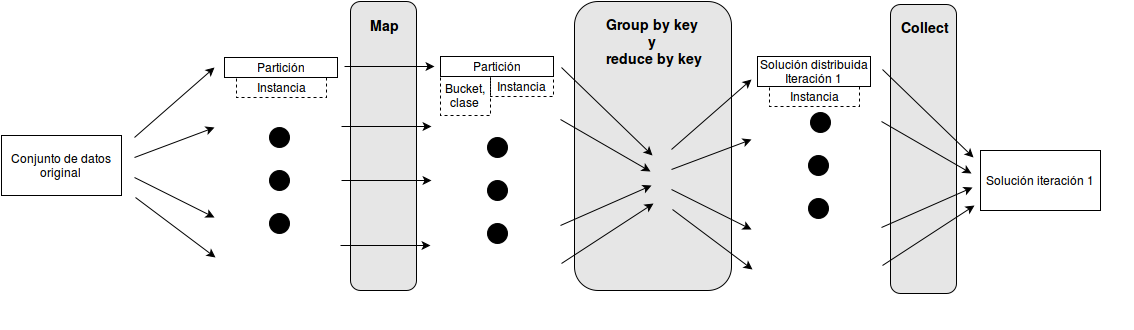
\includegraphics[width=1.0\textwidth]{img/memoria/diagram_LSHIS1}
		\caption{Diagrama de la ejecución del algoritmo LSHIS durante su primera iteración.}\label{fig:img/memoria/diagram_LSHIS1}
	\end{figure}
	\FloatBarrier
	
		\begin{figure}[!h]
		\centering
		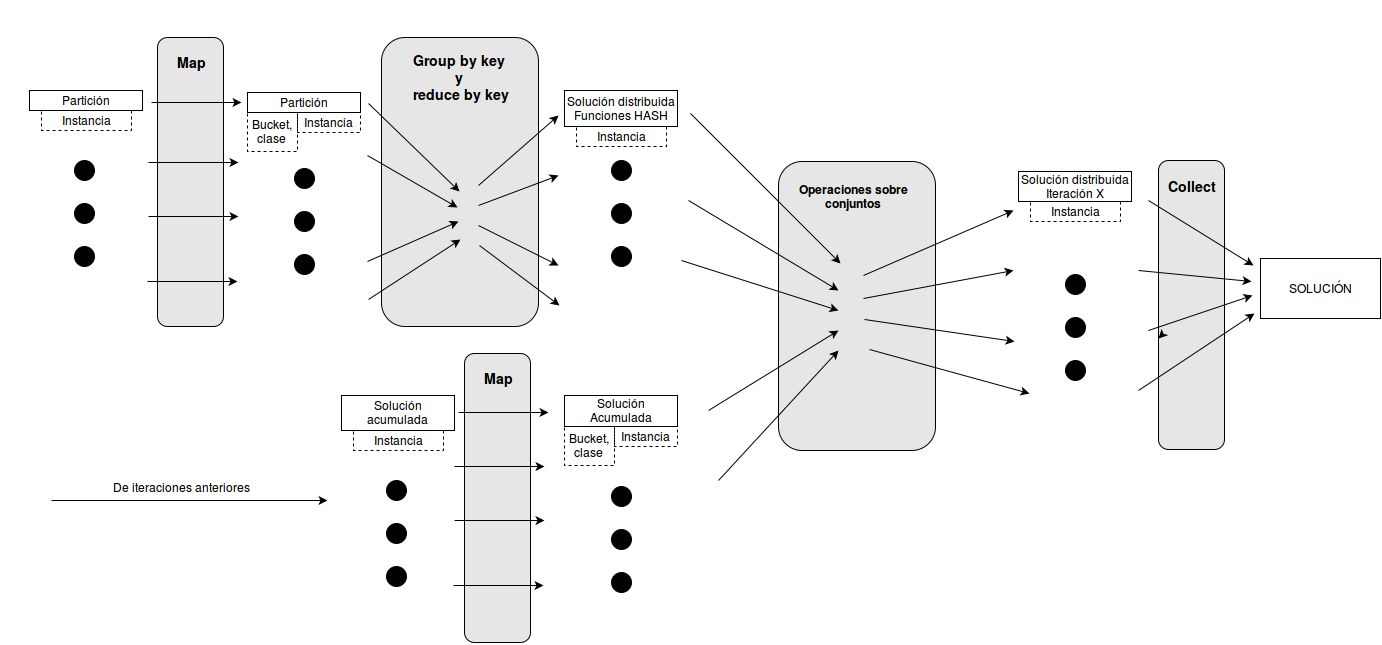
\includegraphics[width=1.0\textwidth]{img/memoria/diagram_LSHIS2}
		\caption{Diagrama de la ejecución del algoritmo LSHIS durante su segunda iteración y sucesivas.}\label{fig:img/memoria/diagram_LSHIS2}
	\end{figure}
	\FloatBarrier

%\imagen{img/memoria/diagram_LSHIS1}{Diagrama de la ejecución del algoritmo LSHIS durante su primera iteración.}
%\imagen{img/memoria/diagram_LSHIS2}{Diagrama de la ejecución del algoritmo LSHIS durante su segunda o mayor iteración.}


\subsection{Implementación concreta de DemoIS}

La implementación de este algoritmo no ha requerido modificar el pseudocódigo del mismo (ver algoritmo \ref{sec:defDemoIS}) pero sí existen varios detalles que conviene destacar sobre la actual implementación.

En primer lugar, como puede apreciarse en la figura \ref{fig:img/memoria/diagram_DemoIS}, no todo el algoritmo se ejecuta en paralelo. A la hora de calcular el \textit{fitness} óptimo lo hacemos de manera secuencial. Esto es así porque no contamos con una implementación paralela del algoritmo KNN, necesario para este proceso (ver \ref{sec:ImplRecursosAdicionales}). Aún con esto, durante esa etapa del proceso solo seleccionamos un pequeño grupo de instancias en comparación con el conjunto inicial, por lo que operar con tal número de datos no supone un problema de rendimiento tan grande.

Existen otras consideraciones de cara a la implementación, como el uso de un particionador aleatorio que no genera particiones del mismo tamaño o la creación de una clase individual que evite la serialización completa del algoritmo al realizar la primera operación \textit{map}. Sin embargo, estos temas serán tratados con más detenimiento en el anexo incluido junto con la memoria.

%En segundo lugar, el particionado del conjunto de datos inicial para realizar las votaciones es aleatorio y genera particiones que no son estrictamente del mismo tamaño, sino que presentan ligeras variaciones de unas a otras. Esto es así porque, en un entorno paralelo, es muy complicado redistribuir las instancias entre los nodos de manera aleatoria pero, a la vez, generando particiones de tamaño similar (y, es por ello, que Spark no proporciona ningún tipo de clase o ayuda en este aspecto). Dado que estos algoritmos están pensados para su ejecución con un número muy grande de instancias, se confía en que la aleatoriedad sitúe un número muy similar de instancias en cada una de las particiones.

	\begin{figure}[!h]
		\centering
		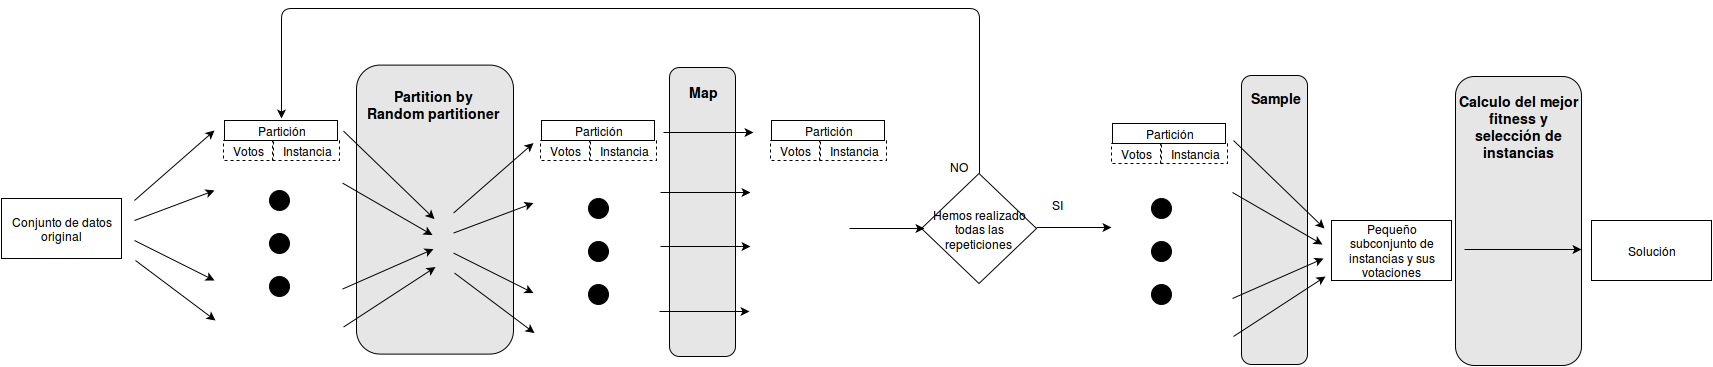
\includegraphics[width=1.0\textwidth]{img/memoria/diagram_DemoIS}
		\caption{Diagrama de la ejecución del algoritmo DemoIS.}\label{fig:img/memoria/diagram_DemoIS}
	\end{figure}
	\FloatBarrier

%\imagen{img/memoria/diagram_DemoIS}{Diagrama de la ejecución del algoritmo DemoIS.}

\section{Comparativa entre las implementaciones de Weka y Spark}

Como otro de los objetivos principales del proyecto, se procedió a realizar una comparación entre nuestras implementaciones de los algoritmos de selección de instancias con las ya existentes para su uso en Weka.

De nuevo, la finalidad de esta comparación tenía varios objetivos: evaluar el rendimiento entre ambas aproximaciones, comprobar el correcto funcionamiento de los algoritmos y evaluar como los cambios de implementación podían haber afectado a su funcionalidad.

Existe una sección más detallada donde se profundizará sobre todos los aspectos relacionados con la comparativa en la sección...

\todo{Incluir pequeña conclusión del resultado, con gráfica si es posible}


\section{Implementación de un entorno gráfico}

En la etapa final, se vio como el proyecto había alcanzado una complejidad considerable en cuando a las opciones de lanzamiento se refiere. Este hecho hacía de la ejecución por línea de comandos un método de lanzamiento mucho más tedioso de lo que a un usuario normal podría resultarle ya de principio. Es por esta razón que, con la intención de facilitar el uso de la biblioteca, se decidió la implementación de una pequeña interfaz gráfica que hiciese más intuitívo el uso del proyecto.

Así pues, se ha realizado una interfaz gráfica que permita introducir, mediante campos de texto, todas las opciones necesarias para la ejecución de los algoritmos, así como la posibilidad de seleccionar los diferentes conjuntos de datos o selectores de instancias. Además, posibilita la acción de crear baterías de ejecuciones al dar la opción de indicar más de una configuración de Spark, conjunto de datos y/o filtro a la vez.

Esta interfaz ofrece dos modos de ejecución:

\begin{itemize}
\item Permite ejecutar los algoritmos directamente desde la interfaz gráfica. Es una opción no recomendada si lo que se busca es eficiencia en los tiempos de ejecución pero es una manera sencilla de realizar pruebas en modo local.
\item Permite la compresión, en un archivo de extensión .zip, de todos los conjuntos de datos necesarios para llevar a cabo las ejecuciones y de un archivo .sh generado dinámicamente que permita la ejecución de todas las ejecuciones seleccionadas. Este tipo de operación facilita que el usuario pueda definir todas las operaciones desde su máquina y, posteriormente, pueda trasladarlas de manera sencilla a un servidor más potente donde serán ejecutadas.
\end{itemize}

Despues de la creación y revisión de algunos prototipos no funcionales, la apariencia final del producto evolucionó hasta alcanzar el aspecto que muestra la figura \ref{fig:img/memoria/full_interface}.

\imagen{img/memoria/full_interface}{Apariencia final de la interfaz gráfica del proyecto.}


\begin{comment}
\section{Comparativa entre las ejecución de clasificadores en Weka y Spark}


Para realizar las mediciones utilizaremos conjuntos de datos de diferentes tamaños (detallados en la sección \ref{Datasets}), pero siempre un mismo algoritmo: el Naive Bayes. Naive Bayes es un algoritmo de clasificación probabilístico y relativamente simple que ya se encontraba implementado tanto en la librería de Weka como en la de Spark, razón por la cual ha sido elegido. En un principio hemos supuesto que no habría grandes diferencias en cuanto a tiempo de ejecución o recursos entre ambas implementaciones.

La ejecución del algoritmo se analizará tanto en Weka como en Spark, siendo en este último ejecutado con diferente número de hilos: 1, 2 y 4.

El programa utilizado para medir el rendimiento ha sido JConsole (ver \ref{DefJConsole}) en ambos casos, con el fin de utilizar la misma herramienta de monitorización en todos los experimientos.
Para observar el comportamiento de los hilos hemos utilizado la herramienta JvisualVM. (ver \ref{DefJvisualVM})

\subsection{Criterios comparados}

Los aspectos que hemos tenido en cuenta a la hora de recoger datos han sido:

\begin{itemize}
	\item \textbf{Tiempo de ejecución:} El periodo analizado es aquel que incluye la lectura de datos, la preparación, entrenamiento y prueba de los diferentes clasificadores que genere la validación cruzada y el cálculo del resultado final. Esta manera de medir es algo que afecta esencialmente a Spark, que lanza un gran número de procesos al iniciarse y pierde algo de tiempo con respecto a Weka.
	\item \textbf{Memoria:} Media del espacio de memoria RAM que consume la ejecución del algoritmo.
	\item \textbf{Porcentaje de CPU:} Media del porcentaje de CPU utilizado con respecto a la potencia total de la CPU. Estas pruebas han sido realizadas sobre una máquina con capacidad para soportar 4 hilos al mismo tiempo, por lo que el uso completo de uno de los hilos supondría un porcentaje de carga de la CPU del 25\% con respecto al total, el uso exclusivo de dos hilos sería un 50\% y así sucesivamente.
	\item \textbf{Comportamiento de los hilos:} Como actúan los hilos del programa cuando se ejecuta el clasificador. Al ser un elemento que no puede medirse directamente, se recurrirá a hablar de él en la sección \ref{ConclusionesWekaSpark} para sustentar otros argumentos, incluyendo imágenes que muestren el comportamiento en el caso de necesitarlas.
\end{itemize}

\subsection{Entorno de las pruebas}

Las mediciones se han llevado a cabo bajo las siguientes circunstancias:

\begin{itemize}
	\item Las ejecuciones se realizaron desde la terminal, tanto en el caso de Weka como en el de Spark.
	\item En todas las ejecuciones hemos contado con memoria suficiente como para poder incluir en ella todo el conjunto de datos. Es necesario destacar que, pese a todo, este supuesto no es común dentro de la minería de datos..
	\item Se necesita un tiempo para indicar a la herramienta de monitorización qué proceso ha de medir. Por ello, con la intención de tener tiempo para asociar la herramienta de monitorización al proceso concreto, la ejecución hilo principal es suspendida durante un pequeño periodo de tiempo antes de iniciar siquiera la lectura de datos del fichero.
	\item Aunque no estamos interesados en la salida final del algoritmo, queremos simular que se realizan las fases de validación y test. No se ha utilizado un archivo diferente como conjunto de test, sino que hemos utilizado una validación cruzada de 10 iteraciones.
	\item El formato utilizado en los ficheros que contienen datos ha sido .arff para Weka y .csv para Spark. La razón por la que no se han utilizado ficheros .csv en Weka ha sido por la posibilidad de que esto produzca errores a la hora de leer el archivo~\cite{CSVWeka}.
	\item El formato de los datos de los conjuntos de datos también ha sufrido variaciones. Mientras que los archivos .arff utilizados por Weka contienen los datos tal y como los proporciona el data set original, algunos conjuntos de datos han tenido que ser normalizados al transformarlos a .csv para poder ser utilizados en Spark. La razón es que el algoritmo NaiveBayes implementado en Spark no admite atributos negativos. Ha afectado a los conjuntos de datos ``Human Activity Recognition'', ``Covertype'' y ``HIGGS''(ver \ref{Datasets}) 
	\item En lo que se refiere a Spark, se ha creado objeto en Scala que es capaz de leer el conjunto de datos, crear diferentes \textit{folds} de dicho conjunto, entrenar y probar el clasificador y mostrar un resultado final. Weka ya proporciona herramientas de este tipo y por lo tanto no ha sido necesario generar ninguna otra clase.
	
\end{itemize}

\todo{Si se puede, se debería indicar el periodo que pasa entre las mediciones de RAM y de CPU}

\subsection{Conjuntos de datos}\label{Datasets}

Los conjuntos de datos, ordenados de menor a mayor según los recursos utilizados para correr el programa, han sido los siguientes:

\tablaSmall{Conjuntos de datos utilizados para la comparación entre Weka y Spark.}{m{5.55cm} >{\raggedleft\let\newline\\\arraybackslash\hspace{0pt}}m{2.35cm} m{2.35cm} m{2.35cm}}{ConjuntosWekaSpark}
{\centering Nombre del conjunto & \centering Instancias & \centering Atributos  & \multicolumn{1}{c}{Clases} \\}{

\centering Iris & 150 & \centering 4 & \multicolumn{1}{c}{3}  \\ [0.2cm]
\centering Human Activity Recognition \cite{HumanActivityDataset} & 165.632 & \centering 17 & \multicolumn{1}{c}{5}   \\ [0.2cm]
\centering Poker \cite{Lichman:2013} & 1.025.010 & \centering 10 & \multicolumn{1}{c}{10}  \\ [0.2cm]
\centering Covertype \cite{Lichman:2013} & 581.012 & \centering 54 & \multicolumn{1}{c}{6}  \\ [0.2cm]
\centering HIGGS \cite{Lichman:2013} \cite{HIGGSDataSet} & 1.469.873 y 2.939.746\tablefootnote{El conjunto original consta de 11.000.000 instancias, pero he reducido su tamaño original para acercarlo más al tamaño de los otros conjuntos.} & \centering 28 & \multicolumn{1}{c}{2} \\ [0.2cm]

} 
\todo{Revisar el código de la tabla}

Indicar que, a la hora de seleccionar los conjuntos, se han elegido aquellos que compartan algunas características comunes:

\begin{itemize}
	\item No existen campos de tipo texto. La única excepción la encontramos en los atributos de clase en los ficheros .arff, pero estos atributos serán tratados como nominales a la hora de la clasificación en Weka.
	\item No existen campos vacíos en ninguna de las instancias de los atributos.
\end{itemize}

\subsection{Resultados}

Los resultados obtenidos han sido agrupados según el conjunto de datos utilizado.

Las pruebas han sido ejecutadas bajo una validación cruzada de 10 x 2, de manera que podamos comprobar si el resultado obtenido se encuentra dentro de lo esperado o su buen/mal funcionamiento se debe a una circunstancia puntual. 

\todo{Replantear tablas de resultados. Crear una sola tabla}

\tablaSmall{Rendimiento sobre el conjunto de datos Iris.}{l c c c c}{RendimientoIris}
{\multicolumn{1}{c}{Criterio} & Weka & Spark 1 hilo & Spark 2 hilos  & Spark 4 hilos \\}{

 Tiempo (s) & 0,1 & 1,97 & 2,13 & 2,15 \\ [0.2cm]
 Memoria (MB)\tablefootnote{\label{noteIris}Los datos de las mediciones sobre el uso de memoria y CPU en el conjunto Iris no son concluyentes debido al corto periodo de tiempo que tardan en ejecutarse.} & - & - & - & - \\ [0.2cm]
 CPU (\%)\footref{noteIris} & - & - & - & - \\ [0.2cm]

}

\tablaSmall{Rendimiento sobre el conjunto de datos Human Activity Recognition.}{l c c c c}{RendimientoHAR}
{\multicolumn{1}{c}{Criterio} & Weka & Spark 1 hilo & Spark 2 hilos  & Spark 4 hilos \\}{

 Tiempo (s) & 12,37 & 16,13 & 11,75 & 11,71 \\ [0.2cm]
 Memoria (MB) & 242,01 & 173,80 & 219,75 & 219,17 \\ [0.2cm]
 CPU (\%) & 25,5 & 36,02 & 54,03 & 59,43\\ [0.2cm]

}

\tablaSmall{Rendimiento sobre el conjunto de datos Poker.}{l c c c c}{RendimientoPoker}
{\multicolumn{1}{c}{Criterio} & Weka & Spark 1 hilo & Spark 2 hilos  & Spark 4 hilos \\}{

 Tiempo (s) & 73,90 & 47,44 & 31,84 & 30,77  \\ [0.2cm]
 Memoria (MB) & 424,65 & 162,93 & 243,76 & 255,11\\ [0.2cm]
 CPU (\%) & 30,05 & 29,41 & 51,22 & 55,68 \\ [0.2cm]

}

\tablaSmall{Rendimiento sobre el conjunto de datos Covertype.}{l c c c c}{RendimientoCovertype}
{\multicolumn{1}{c}{Criterio} & Weka & Spark 1 hilo & Spark 2 hilos  & Spark 4 hilos \\}{

 Tiempo (s) & 183,95 & 101,91 & 73,23 & 53,78 \\ [0.2cm]
 Memoria (MB) & 576,78 & 177,37 & 213,7 & 211,7\\ [0.2cm]
 CPU (\%) & 28,17 & 28,26 & 43,10 & 71,94 \\ [0.2cm]

}

\tablaSmall{Rendimiento sobre el conjunto de datos HIGGS (1.469.873 instancias).}{l c c c c}{RendimientoHIGGS1}
{\multicolumn{1}{c}{Criterio} & Weka & Spark 1 hilo & Spark 2 hilos  & Spark 4 hilos \\}{

 Tiempo (s) & 246,97 & 191,9 & 130,37 & 99,2 \\ [0.2cm]
 Memoria (MB) & 832,88 & 872,56 & 864,92 & 921,49 \\ [0.2cm]
 CPU (\%) & 28,60 & 26,64 & 49,91 & 89,24\\ [0.2cm]

}

\tablaSmall{Rendimiento sobre el conjunto de datos HIGGS (2.939.746 instancias).}{l c c c c}{RendimientoHIGGS2}
{\multicolumn{1}{c}{Criterio} & Weka & Spark 1 hilo & Spark 2 hilos  & Spark 4 hilos \\}{

 Tiempo (s) & 503,929 & 368,721 & 264,023 & 215,214\\ [0.2cm]
 Memoria (MB) & 1747,22  & 883,28 & 911,77 & 853,58 \\ [0.2cm]
 CPU (\%) & 29 & 26,37 & 50,74 & 91,58 \\ [0.2cm]

}

\subsection{Conclusiones}\label{ConclusionesWekaSpark}
\todo{¿Mover esta sección al final de la memoria?}
\todo{Revisar las referencias ante un cambio de tabla de resultados.}
\begin{itemize}
	\item Puede observarse claramente que Weka es considerablemente superior a Spark cuando utilizamos conjuntos de datos pequeños, como observamos en la tabla \ref{tabla:RendimientoIris} o incluso en la tabla \ref{tabla:RendimientoHAR}, pero su rendimiento se ve superado con notable diferencia cuando el conjunto de datos empieza a sobrepasar las 100.000 instancias de Human Activity Recognition (ver \ref{Datasets}).
	\item Salvo cuando tratamos con conjuntos de datos pequeños, vease por ejemplo la tabla \ref{tabla:RendimientoIris}, el rendimiento del algoritmos Naive Bayes de Weka es menor si lo comparamos con las ejecuciones sobre un solo hilo de Naive Bayes en Spark. Es posible que una de las causas sea la diferente implementación del algoritmo en Weka y en Spark.
	\item Como era de esperar, doblar el número de hilos no implica reducir a la mitad el tiempo de procesamiento, sino que genera un beneficio menor que, en algún momento y dependiendo del tamaño del conjunto de datos analizado, dejará de ser significativo aunque sigamos añadiendo hilos.
	\missingfigure{Probablemente incluya una gráfica sobre el rendimiento de Spark sobre HIGGS}
	\item Generalmente Spark necesita menos memoria que Weka para ejecutar el programa.
	\item Parece que el porcentaje de RAM requerido por Spark aumenta ligeramente cuantos más hilos tengamos en ejecución, algo que se aprecia bien en los conjuntos de datos pequeños.
	\item El porcentaje de uso de la CPU en Weka se situa siempre entorno a los valores 25-30\%. Esto es así porque la ejecución de todas las tareas es lineal, consumiendo únicamente un hilo de los 4 que posee la máquina en la que se están realizando las prueba.
	\item Vemos que el porcentaje de uso de la CPU en las diferentes pruebas con Spark suele corresponder al número de hilos con los que se lanza la aplicación: 25\% para un hilo, 50\% para dos y, teóricamente, 90-100\% para 4. Sin embargo, y como podemos apreciar en las tablas \ref{tabla:RendimientoPoker} o \ref{tabla:RendimientoCovertype}, la ejecución con cuatro hilos no aprovecha al máximo las capacidades del procesador cuando el conjunto de datos es pequeño. Observando más de cerca el evento, vemos que, independientemente del número de hilos que decimos a Spark que maneje, en estos conjuntos de datos únicamente se lanzan dos hilos como máximo. Atribuimos esto a un comportamiento propio de Spark, que evalua que no existe necesidad de manejar tantos hilos de ejecución. 
	\missingfigure{Incluir comportamiento de los hilos de jvisualvm}
\end{itemize}


\section{Comparativa entre la ejecución del algoritmo LSHIS en Spark y Weka}

\subsection{Criterios comparados}

Se ha realizado la comparación teniendo en mente la medición de los siguientes parámetros:

\begin{itemize}
	\item \textbf{Reducción del conjunto de datos:} Relación entre el tamaño del conjunto de datos original y el obtenido tras la aplicación del algoritmo.
	\item \textbf{Tiempo de ejecución:} Tiempo real que ha requerido la ejecución del algoritmo LSHIS.
	\item \textbf{Precisión de un clasificador con el nuevo conjunto:} Porcentaje de acierto en test al aplicar el algoritmo KNN (K-Nearest neighbors) sobre el nuevo conjunto de datos.
\end{itemize}
\subsection{Entorno de las pruebas}
\begin{itemize}
	\item Las pruebas han sido ejecutadas bajo una validación cruzada de 10 x 2. \todo{ En la comparación de arriba esto está en otro sitio.}
		\item Todos los conjuntos de datos han sido normalizados
\end{itemize}

\subsection{Conjuntos de datos}

\todo{Esto ya esta arriba}

\subsection{Resultados}

\tablaSmall{Comparativa de LSHIS sobre el conjunto de datos Iris.}{l c c c c}{CompIrisLSHIS}
{\multicolumn{1}{c}{Criterio} & Weka & Spark 1 Ejecutor & Spark 2 Ejecutores  & Spark 4 Ejecutores \\}{

 Instancias & 22 & 26 & 23 & 22 \\ [0.2cm]
 Tiempo(s) & 12 & 3340 & 2670 & 10574 \\ [0.2cm]
 Acierto(\%) & 92 & - & - & - \\ [0.2cm]

}

\tablaSmall{Comparativa de LSHIS sobre el conjunto de datos Human Activity.}{l c c c c}{CompHALSHIS}
{\multicolumn{1}{c}{Criterio} & Weka & Spark 1 Ejecutor & Spark 2 Ejecutores  & Spark 4 Ejecutores \\}{

 Instancias & 147 & 350 & 340 & 367 \\ [0.2cm]
 Tiempo(s) & 167 & 9919 & 12327 & 22525 \\ [0.2cm]
 Acierto(\%) & 57,1 & 71,95 & 69,21 & 69,4 \\ [0.2cm]

}


\tablaSmall{Comparativa de LSHIS sobre el conjunto de datos Poker.}{l c c c c}{CompPokerLSHIS}
{\multicolumn{1}{c}{Criterio} & Weka & Spark 1 Ejecutor & Spark 2 Ejecutores  & Spark 4 Ejecutores \\}{

 Instancias & 3806 & 7545 & 7613 & 7625 \\ [0.2cm]
 Tiempo(s) & 823 & 24057 & 19448 & 26464 \\ [0.2cm]
 Acierto(\%) & 26,13 & 27,14 & 31,26 & 30,62 \\ [0.2cm]

}


\tablaSmall{Comparativa de LSHIS sobre el conjunto de datos Covertype.}{l c c c c}{CompCovLSHIS}
{\multicolumn{1}{c}{Criterio} & Weka & Spark 1 Ejecutor & Spark 2 Ejecutores  & Spark 4 Ejecutores \\}{

 Instancias & 2317 & 3987 & 3969 & 3982 \\ [0.2cm]
 Tiempo(s) & 570 & 24527 & 22157 & 27262 \\ [0.2cm]
 Acierto(\%) &  &  &  &  \\ [0.2cm]

}

\tablaSmall{Comparativa de LSHIS sobre el conjunto de datos HIGGS. (1.469.873 instancias)}{l c c c c}{CompHIGGS1LSHIS}
{\multicolumn{1}{c}{Criterio} & Weka & Spark 1 Ejecutor & Spark 2 Ejecutores  & Spark 4 Ejecutores \\}{

 Instancias &  &  &  &  \\ [0.2cm]
 Tiempo(s) &  &  &  &  \\ [0.2cm]
 Acierto(\%) &  &  &  &  \\ [0.2cm]

}

\tablaSmall{Comparativa de LSHIS sobre el conjunto de datos HIGGS. (2.939.746 instancias)}{l c c c c}{CompHIGGS2LSHIS}
{\multicolumn{1}{c}{Criterio} & Weka & Spark 1 Ejecutor & Spark 2 Ejecutores  & Spark 4 Ejecutores \\}{

 Instancias &  &  &  &  \\ [0.2cm]
 Tiempo(s) &  &  &  &  \\ [0.2cm]
 Acierto(\%) &  &  &  &  \\ [0.2cm]

}



\subsection{Conclusiones}

\begin{itemize}
	\item No se puede predecir la salida de Spark por ser la ejecución en paralelo.
	\item Con tan poca carga de trabajo, Weka es mucho mejor. A partir de Poker podemos ver que Spark empieza a funcionar un poco como debería, donde 2 ejecutores funcionan mejor que 1, pero nunca llegamos a necesitar los 4 cores.
	\item
\end{itemize}


\end{comment}
\capitulo{6}{Trabajos relacionados}

%Este apartado sería parecido a un estado del arte de una tesis o tesina. En un trabajo final grado no parece obligada su presencia, aunque se puede dejar a juicio del tutor el incluir un pequeño resumen comentado de los trabajos y proyectos ya realizados en el campo del proyecto en curso. 

\section{Weka}

Aunque ya ha sido mencionado y definido con anterioridad en esta memoria (ver sección \ref{sec:DefWeka}), parece obligatoria una mención a dicho programa en este apartado.

Cabe destacar que, aunque tanto Weka como este proyecto comparten un objetivo común como es el de presentar una biblioteca con algoritmos de minería de datos y hacerlo de manera que sea fácil su utilización, el ámbito de aplicación de ambos programas es completamente distinto. Mientras que Weka parece pensado enfocado a pequeños/medianos conjuntos de datos y una ejecución secuencial de sus algoritmos, este proyecto utiliza Spark para hacer factible la idea de aplicar algoritmos demasiado costosos como para ser ejecutados con grandes conjuntos de datos en una sola máquina.

\section{Knowledge Extraction based on Evolutionary Learning (KEEL)}

KEEL \cite{KEELSoft1,KEELSoft2} es una herramienta de minería de datos basada en Java que permite la aplicación, sobre conjuntos de datos, de algoritmos de extracción de conocimiento. Al igual que Weka, también posibilita la opción de aplicar métodos de pre procesamiento sobre los datos originales antes de que sean utilizados en las labores de minería.

La diferencia fundamental de este software, con respecto al presentado a lo largo de la memoria, vuelve a ser, de nuevo, la ejecución secuencial de algoritmos de KEEL con respecto a la ejecución paralela de Spark.

\section{Documentos científicos de LSHIS y DemoIS}

A lo largo del proyecto, y en especial todo lo relacionado con la implementación y prueba de los algoritmos, se ha contado con los documentos científicos que definían la implementación y uso de LSHIS y DemoIS. Dichos documentos, ya mencionados anteriormente en la memoria, han sido ``LSH-IS: Un nuevo algoritmo de selección de instancias de complejidad lineal para grandes conjuntos de datos''\cite{LSHISPaper} y ``Democratic instance selection: A linear complexity instance selection algorithm based on classifier ensemble concepts''\cite{DemoISPaper}.

Ambos documentos, además de contener información sobre los algoritmos implementados, también contienen comparaciones de rendimiento con otras alternativas de selección de instancias. En lo que se refiere a este proyecto, las pruebas realizadas han tenido como objetivo la comparativa entre tiempos de ejecución de las implementaciones secuencial y paralela, por lo que podemos defender que se han evaluado aspectos diferentes durante la etapa de experimentación.

Además, se ha contado con la implementación de los algoritmos LSHIS y DemoIS para su ejecución en Weka \cite{arnaiz2012herramienta}, lo que ha posibilitado realizar las experimentaciones defendidas en esta memoria y los documentos anexos.

\capitulo{7}{Conclusiones y Líneas de trabajo futuras}

%Todo proyecto debe incluir las conclusiones que se derivan de su desarrollo. Éstas pueden ser de diferente índole, dependiendo de la tipología del proyecto, pero normalmente van a estar presentes un conjunto de conclusiones relacionadas con los resultados del proyecto y un conjunto de conclusiones técnicas. 
%Además, resulta muy útil realizar un informe crítico indicando cómo se puede mejorar el proyecto, o cómo se puede continuar trabajando en la línea del proyecto realizado. 

La realización del proyecto ha permitido comprobar la complejidad de la programación paralela y aplicada a escenarios donde el rendimiento, la comunicación entre unidades de procesamiento o la falta de recursos son aspectos a tener muy en cuenta.

Los objetivos propuestos al comienzo del trabajo se han cumplido, logrando la implementación paralela de varios algoritmos de selección de instancias y su posterior comparación con las implementaciones anteriores. Igualmente, otras metas definidas \textit{a posteriori}, como la implementación de una interfaz gráfica y la ejecución en la nube, han sido correctamente cumplidas.

Finalmente, y centrándonos en el ámbito de las comparaciones, este proyecto nos han ayudado a desmentir la hipótesis inicial con la que se comenzó a trabajar: que todos los algoritmos propuestos conseguirían reducir el tiempo de ejecución con respecto a sus antiguas versiones. Se ha visto como el algoritmo LSHIS, debido a su rapidez, es difícil de mejorar cuando intentamos paralelizarlo. Por el contrario, el algoritmo DemoIS muestra resultados muy favorables incluso con conjuntos de instancias pequeños.


\subsection{Lineas de trabajo futuras}
La propia naturaleza del proyecto ofrece una gran variedad de alternativas para seguir trabajando:

\begin{itemize}
\item \textbf{Continuar trabajando sobre los algoritmos ya implementados:} Aunque es posible que el algoritmo LSHIS pueda ser abordado utilizando un paradigma distinto (\textit{streaming}), DemoIS todavía puede ofrecer un gran margen de mejora. Una implementación paralela del algoritmo K-NN o una nueva estrategia para la creación de subconjuntos podrían suponer, no solo una mejora en el comportamiento del algoritmo, sino también una todavía más rápida ejecución. Además, existen algunas variaciones de los algoritmos que no han sido implementadas en su versión paralela.

\item \textbf{Continuar las mediciones en la nube:} Aunque se han realizado numerosos experimentos para comprobar el rendimiento de los algoritmos propuestos, la mayoría de ellos se han realizado en una única máquina, limitando nuestros recursos o el tamaño de los conjuntos de datos a utilizar. Es cierto que se han realizado algunas pruebas en otro tipo de entornos, pero se han visto limitadas por problemas técnicos. Realizar más mediciones en un auténtico clúster permitiría realizar comparaciones con conjuntos de datos mucho más grandes, bastantes más recursos, y probablemente ayudase a definir más claramente el alcance del paradigma de programación en paralelo.

\item \textbf{Mejorar métodos de lectura/escritura:} Un aspecto que no ha sido tratado durante este proyecto ha sido la manera en la que leer o almacenar los conjuntos de datos. Técnicas como la lectura de datos de un sistema de ficheros distribuido o de una base de datos podrían ser de mucha utilidad en este área y, por lo tanto, podrían ser abordados en futuras mejoras.

\item \textbf{Seguir ampliando el número de algoritmos de minería de datos:} La estructura del proyecto y el campo en el que se desarrolla, dejan la puerta abierta a la implementación de multitud de algoritmos que se ejecuten en paralelo, pues no existe actualmente una gran librería que cubra este ámbito.


\end{itemize}





\bibliographystyle{plain}
\bibliography{bibliografia}

\end{document}
